%! Author = vladimir
%! Date = 05/02/21

% Preamble
\documentclass[12pt]{article}

% Packages
\usepackage{amsmath}
\usepackage[spanish,activeacute]{babel}
\usepackage{setspace}
\usepackage{biblatex}
%---------------- Marco del doc y separacion entre lineas -----------------
\usepackage[a4paper]{geometry}
\geometry{top= 1 in,bottom = 1 in , left = 1 in, right = 1 in}
\doublespacing
%\geometry{top=2cm, bottom=2.0cm, left=2.5cm, right=2cm}
%- \linespread{1.3}

%--- bibiliografia
\addbibresource{bibliography/Watkins.bib}
\addbibresource{bibliography/Gulumbic2021.bib}
\addbibresource{bibliography/Anan.bib}
\addbibresource{bibliography/Pranav.bib}


%----- Para no poner sangria ----------------
\setlength{\parindent}{0cm}

%-- para las imagenes
\usepackage{graphicx}
\usepackage{float}
\usepackage{hyperref}
\graphicspath{ {./images/} }

%-- comandos personalizados
\newcommand{\bigo}{\mathcal{O}}

\usepackage{dirtree}

% Title
\title{ Dos algoritmos para resolver el Problema del Recorrido del Caballo
    utilizando Prolog.}
\author{Sierra Casiano Vladimir}

% Document
\begin{document}

    \maketitle

    \begin{abstract}
        Para el presente proyecto se abordar'a una variante del Problema del Recorrido del
        Caballo.
        Se presentar'an dos maneras (a comparar) para encontrar soluciones
        'optimas, la primera es utilizando la regla de Warnsdorff, y la segunda
        es adaptando el algoritmo bioinspirado Artificial Bee Colony. Ambas
        soluciones tendr'an un enfoque declarativo.
    \end{abstract}


    \section{Preliminares.}

    \subsection{Problema del Recorrido del Caballo.}


    El problema data a mediados del Siglo VI en la India \cite{watkins} (muy cerca del
    origen del ajedrez) y ha sido muy estudiado a lo largo de la historia por
    celebres matem'aticos como
    Euler, quien enunci'o el problema de la siguiente manera:
    \textit{ ?`C'omo se pueden encontrar todas las secuencias de movimientos de
    la pieza del caballo en un tablero de ajedrez de tal manera que cada casilla del
    tablero es visitada exactamente una vez?
    }  \cite{golumbic2021} \\
    El problema es una instancia del m'as general
    Problema del camino Hamiltoniano de la  Teor'ia de Gr'aficas.

    A lo largo del tiempo varios enfoques han sido propuestas para
    encontrar soluciones tales como la fuerza bruta, divide y vencer'as,
    b'usqueda DFS con backtracking e incluso redes neuronales \cite{anan}.
    El problema es NP-completo, por lo que encontrar algoritmos eficientes
    para dar soluciones sigue siendo un reto interesante.



    \subsection{Definici'on del problema.}
    La pieza del caballo en el ajedrez tiene un movimiento en forma de \textit{L} , como
    se ilustra a continuaci'on.
    
    \begin{figure}[H]
        \centering
        \fbox{
            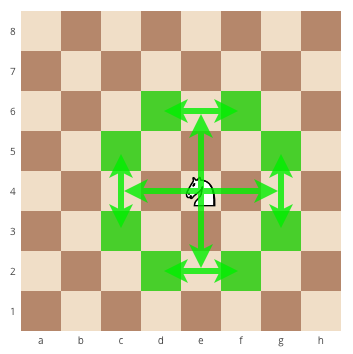
\includegraphics[scale = 0.6]{knight_move.png}
        }
        \caption{Posibles movimientos para el caballo.}
        \label{fig:knight_move}
    \end{figure}



    El problema que queremos resolver es, dada una posici'on inicial y el tama'no del tablero,
    encontrar el camino m'as largo posible utilizando los movimientos del caballo
    y visitando cada casilla a lo m'as una vez.


    \subsection{Artificial Bee Colony.}\label{section:bee_colony}

    El algoritmo Artificial Bee Colony (ABC) fue propuesto en el a'no 2005  por el  Dervis Karaboga,
    y est'a inspirado en el comportamiento de abejas mel'iferas para encontrar fuentes de comida de calidad. Es uno de
    los algoritmos bioinspirados m'as populares para problemas de optimizaci'on num'erica \cite{anan}.
    En esta secci'on describiremos brevemente su funcionamiento.

    \textbf{Componentes.}
    \begin{itemize}
        \setlength\itemsep{0em}
        \item Abejas, que se dividen en tres tipos: empleadas, observadoras y exploradoras.
        \item Se tiene un mismo n'umero de abejas de cada tipo.
        \item Fuentes de comida, que representa una posible soluci'on al problema.
        \item Cada abeja empleada es encargada de una fuente de comida (es decir, tenemos el mismo n'umero de fuentes
                de comida que de abejas empleadas).
        \item Hay una funci'on fitness, que eval'ua la calidad de una fuente de comida.
    \end{itemize}

    \textbf{Metodolog'ia.}
    \begin{itemize}
        \item Se generan fuentes de comida de manera aleatoria.
        \item Se repite un n'umero definido de veces los siguientes pasos
            \begin{itemize}
                \setlength\itemsep{0em}
                \item Todas las abejas empleadas buscan una abeja compa'nera para compartir informaci'on y actualizar
                    la fuente de comida.
                \item Las abejas observadoras toman las fuentes de comida de las abejas empleadas, y seleccionan
                    solo a algunas para actualizar su informaci'on.
                \item Las abejas exploradoras toman las fuentes de comida y las inspeccionan. Si encuentran
                alguna fuente de comida que no puede optimizarse m'as y que se encuentra por debajo de un l'imite
                se descarta y se cambia por una nueva posici'on generada aleatoriamente.

            \end{itemize}

    \end{itemize}

    De manera resumida, las abejas empleadas actualizan todas las fuentes de comida, las observadoras
    actualizan solo algunas soluciones (las m'as optimas al momento) y las exploradoras descartan soluciones
    sub'optimas. Este proceso se repite un n'umero finito de veces y al final observamos
    la soluci'on global.

    \subsection{El papel de la Programaci'on Declarativa.}
    Para las implementaciones de este proyecto se opt'o por el uso de Prolog, lenguaje que pertenece
    al paradigma de la Programaci'on L'ogica. \\
    En Prolog la informaci'on es manejada con hechos y reglas de producci'on.

    Como observaremos en la secci'on ~\ref{section: desarrollo}, una considerable cantidad de operaciones
    que se requieren para los algoritmos desarrollados en este proyecto consisten en
    \begin{itemize}
        \item Verificar que se cumplan condiciones (por ejemplo, para mutar informaci'on).
        \item Explorar varias posibilidades en un mismo punto (por ejemplo, explorar los posibles movimientos).
    \end{itemize}

    Ambas caracter'isticas est'an intimamente ligadas a la filosof'ia de Prolog, que nos regala la exploraci'on a trav'es
    de su 'arbol de resoluci'on y adem'as tiene el bactracking ya implementado. Estos aspectos hacen que una
    implementaci'on en este lenguaje sea atractiva.




    \section{Desarrollo.}\label{section: desarrollo}

    \subsection{Representaci'on de la informaci'on.}
    Para todos los m'etodos propuestos a continuaci'on es importante
    entender c'omo estamos representando los distintos
    elementos.

    \begin{itemize}
        \item La posici'on en el tablero es un par  $\mathbf{(X,Y)}$ , donde
        $X$ es el n'umero de la columna y $Y$ el n'umero del rengl'on.
        Ambos valores est'an en un rango entre $1$ y $N$ (longitud
        del lado del tablero). \\
        Por ejemplo, para un tablero de $3\times 3$ los
        pares para cada posici'on son los siguientes

        \begin{figure}[H]
            \centering
            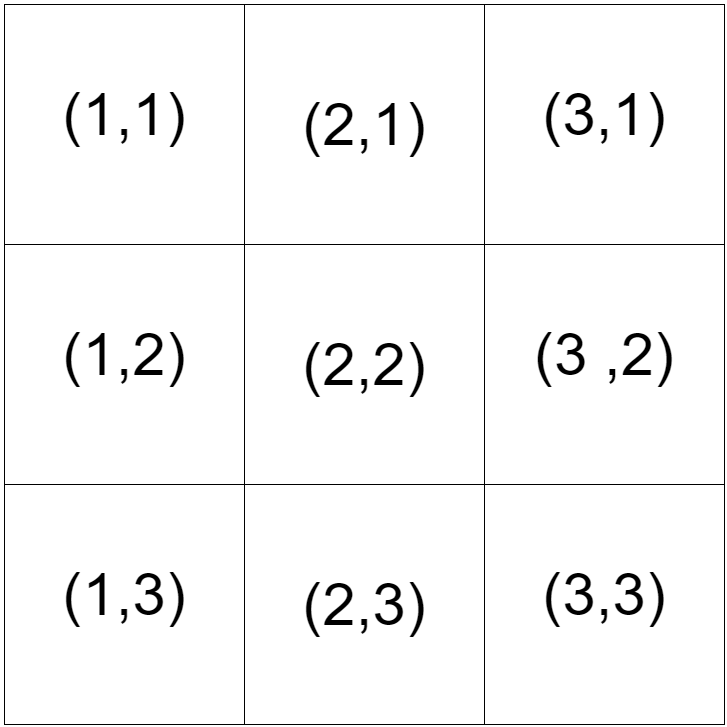
\includegraphics[scale=0.22]{tablero_posiciones.png}
            \caption{Representaci'on de las posiciones en un tablero de $3\times 3$.}
            \label{fig: posiciones}
        \end{figure}



        \item Un recorrido se representa con una lista, donde cada elemento
        es una posici'on del tablero. El orden en que se visitan las
        posiciones se lee de izquierda a derecha en la lista.\\
        Por ejemplo, dado el recorrido

        \begin{figure}[H]
            \centering
            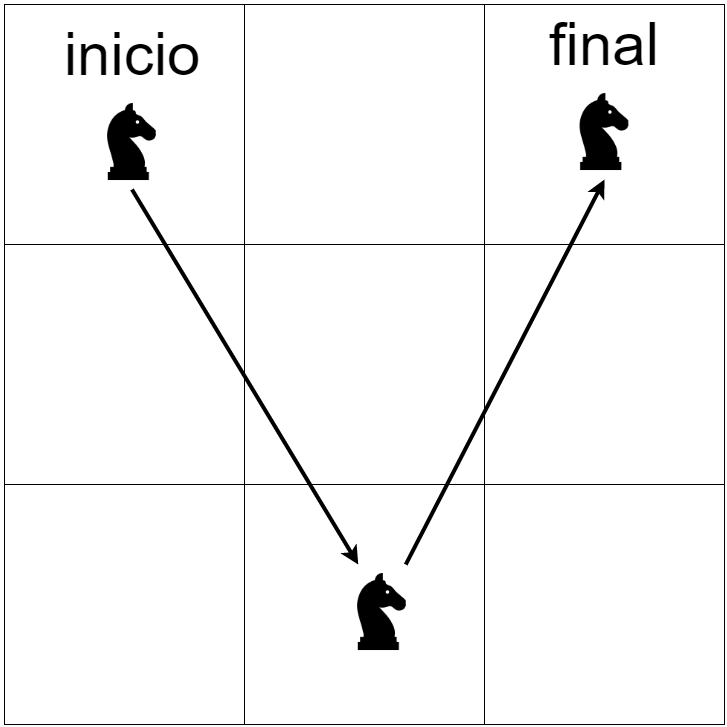
\includegraphics[scale=0.22]{recorrido1.png}
            \caption{Ejemplo de secuencia de movimientos.}
            \label{fig:recorrido1}
        \end{figure}


        su representaci'on es: $[ (1,1) \; ,\; (2,3),\; (3,1) ]$

    \end{itemize}

    Algunos aspectos particulares de cada m'etodo ser'an nombrados
    en su correspondiente secci'on.


    \subsection{Tratando de resolver el problema con fuerza
    bruta.}

    La soluci'on m'as siple en la que podemos pensar es recorrer todos los caminos posibles, y al final elegir
    el m'as largo. Esto se puede hacer utilizando una b'usqueda DFS y backtracking.


    El 'arbol de posibles movimientos y el backtracking es manejado
    gracias a Prolog, pues el recorrido DFS corresponde
    a la exploraci'on que hace Prolog en el 'arbol de resoluci'on. Mientras que el backtracking nos permite volver a posiciones anteriores
    para explorar otro posible camino.

    Potencialmente, tenemos que elegir entre 8 casillas (a las que se puede mover) en cada paso.
    Como el n'umero de casillas es $N^2$  el recorrer todos los caminos tiene una complejidad de
    $\bigo( 8^{N^2} ) $.

    \begin{figure}[H]
        \centering
        \fbox{ 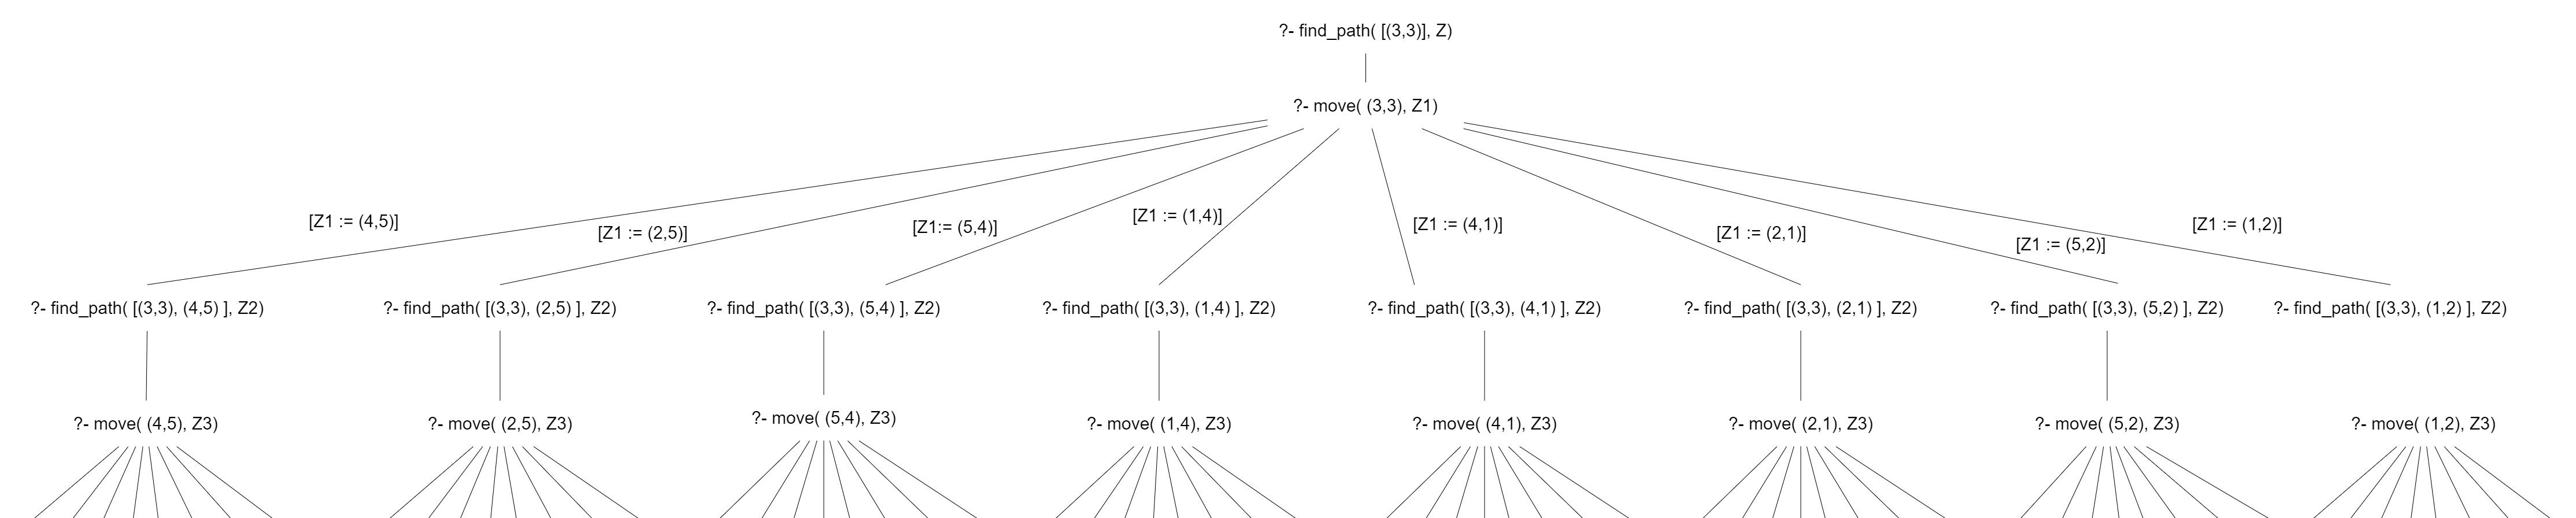
\includegraphics[scale=0.13]{tree1.png} }
        \caption{Primer nivel del 'arbol de b'usqueda para un tablero $5 \times 5$. }
        \label{fig:tree1}
    \end{figure}

    Explorar todos los caminos es inviable, la capacidad de las  computadoras de hoy en d'ia es superada para un tablero
    de $8\times 8$. Para reducir el espacio
    de b'usqueda (y entonces obtener resultados en un tiempo razonable)
    se pueden utilizar muchos m'etodos, uno relativamente
    simple es el descrito en la secci'on siguiente.



    \subsection{Soluci'on con la regla de Warnsdorff.}
    En 1823  H.C. Warnsdorff propus'o una heur'istica muy eficiente para afrontar el problema, a dicha heur'istica se le conoce
    como regla de Warnsdorff \cite{pranav} . Aunque la heur'istica fue propuesta para el problema original (encontrar el camino que pasa por todas
    las casillas) para nuestra variante tambi'en funciona, pues maximiza la longitud de los recorridos.

    Llamamos una casilla adyacente a una casilla a la cual se puede ir desde la posici'on actual con un movimiento del caballo.

    Para decidir el siguiente movimiento primero se observan las casillas adyacentes a la actual, para cada una de ella se obtiene la
    cantidad de casillas adyacentes no visitadas, al final se elige aquella con la menor cantidad.\\
    Entonces el siguiente movimiento debe ser a
    aquella casilla adyacente no vistada que tenga la menos cantidad de casillas adaycentes no visitadas.

    Por ejemplo, en la siguiente imagen la pieza del caballo est'a en su posici'on inicial, sus casillas adyacentes
    tienen el n'umero entero correspondiente a la cantidad de casillas adyacentes no visitadas. El siguiente movimiento siguiendo la regla
    de Warnsdorff es hacia la casilla con el valor 2.

    \begin{figure}[H]
        \centering
        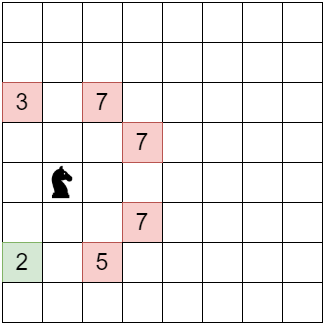
\includegraphics[scale=0.5]{warnsdorff.png}
        \caption{Ejemplo de regla de Warnsdorff.}
        \label{fig:warnsdorff}
    \end{figure}

    El 'arbol de resoluci'on de Prolog entonces ya no tiene que desarrollar las ramas para todos los posibles movimientos, con la heur'istica escogemos solo uno y sobre
    esa rama seguimos desarrollando.

    Por ejemplo, para un tablero de $5 \times 5$ con posici'on inicial $(3,3)$ el desarrollo de los primeros movimientos con la heur'istica
    puede ser observado en el siguiente 'arbol \footnote{El 'arbol de la imagen no muestra todo el desarrollo de Prolog, solo es una versi'on simplificada
    para observar la reducci'on de ramas.}.

    \begin{figure}[H]
        \centering
        \fbox{ 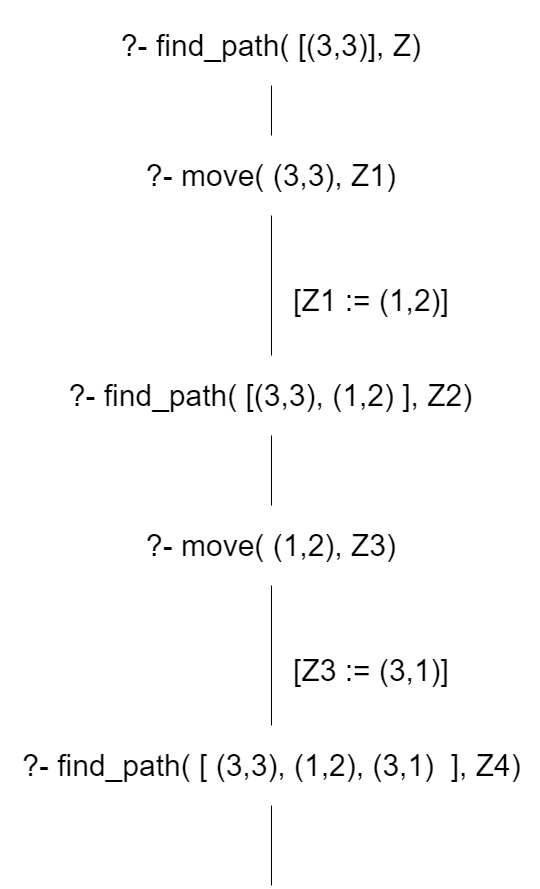
\includegraphics[scale=0.25]{tree2.png} }
        \caption{Primeros tres niveles del 'arbol de b'usqueda con heur'istica.}
        \label{fig:tree2}
    \end{figure}


    \subsection{Adaptando Artificial Bee Colony para resolver el problema.}

    \subsubsection{Representaci'on de las fuentes de comida.}

    El algoritmo ABC est'a planteado originalmente para problemas con valores continuos. Como nuestro problema es discreto
    se deben realizan unas adaptaciones. La siguiente adaptaci'on est'a basada en la propuesta de Banharnsakun \cite{anan}.


    Los 8 patrones de movimiento del caballo se identificar'an con un n'umero:
    \begin{figure}[H]
        \centering
        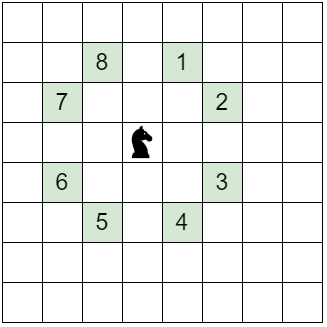
\includegraphics[scale=0.5]{id_move.png}
        \caption{Identificadores de los patrones.}
        \label{fig:id_move}
    \end{figure}



    Las posibles  soluciones para un tablero de $N \times N$
    se representan con una lista de longitud $N^{2} -1 $, donde
    cada elemento de la lista es un n'umero entre $1$ y $8$.

    \begin{figure}[H]
        \centering
        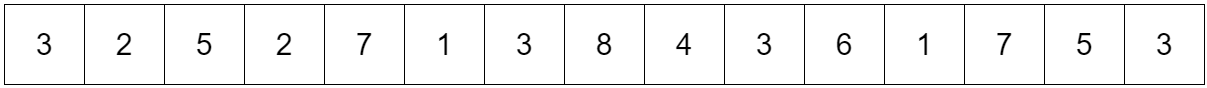
\includegraphics[scale=0.3]{food_source1.png}
        \caption{Ejemplo de posible soluci'on para un tablero de $4\times 4$.}
        \label{fig:food_source1}
    \end{figure}

    El significado operacional de esta secuencia es, dada la posici'on inicial, aplicar el patr'on de movimiento
    que se encuentra en la cabeza de la lista, una v'ez llegada a la posici'on destino aplicar el
    patr'on de movimiento que guarda el siguiente elemento de la lista. \\
    Es claro que las listas pueden guardar movimientos inv'alidos, es decir, al aplicar
    el patr'on de movimiento se regresa a una casilla previamente visitada o se sale del tablero. \\
    El objetivo del algoritmo es entonces maximizar los movimientos v'alidos.


    \subsubsection{Funci'on fitness.}

    La definici'on de nuestra funci'on fitness est'a dada recursivamente:

    \begin{equation} \label{eq: fitness}
        \begin{split}
            f(\; [\;] \;) &= 0 \\
            f( x:xs ) &= \begin{cases}
                            1 + f(xs) &\text{si $x$ es un movimiento v'alido}\\
                            0 &\text{si $x$ es un movimiento inv'alido }
            \end{cases}
        \end{split}
    \end{equation}
    Decimos que la fuente de comida $V_i$ tiene un valor fitness de $f(V_i)$.\\
    Observe que con esta definici'on entre m'as grande es el valor de la funci'on fitness m'as
    largo es el recorrido que representa la lista.

    \subsubsection{Actualizaci'on de las soluciones.}\label{section: merge}

    Para actualizar una fuente de comida $V_{1}$, primero se
    escoge aleatoriamente una fuente de comida distinta $V_{2}$ , el intercambio
    de informaci'on se realiza con tres cortes e intercalando los fragmentos de ambas fuentes, como se ilustra en
    la siguiente imagen:

    \begin{figure}[H]
        \centering
        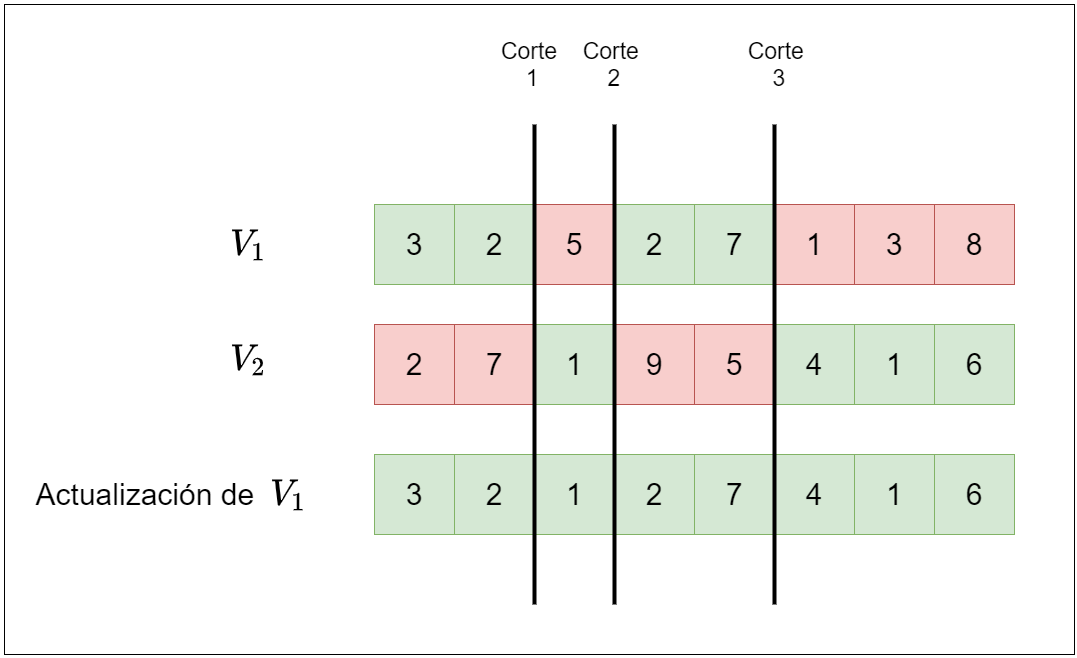
\includegraphics[scale=0.35]{merge.png}
        \caption{Proceso de actualizaci'on de una fuente de comida.}
        \label{fig:merge}
    \end{figure}


    Los puntos de corte son escogidos aleatoriamente.\\
    Recuerde que en todo momento se mantiene una estrategia glotona, cuando una fuente de comida muta se comprueba
    si el valor de la funci'on fitness se incrementa o no, en caso de que no se incremente se descartan los cambios.


    \subsubsection{Algoritmo.}
    Como mencionamos en la secci'on ~\ref{section:bee_colony}, los trabajos realizados por los tres tipos de abejas
    conforman un ciclo de ejecuci'on.

    \textbf{Abejas empleadas.}\\
    Todas las abejas tienen asociada una fuente de comida, de manera aleatoria escogen a una compa'nera y
    actualizan la posici'on de su fuente de comida siguiendo el m'etodo descrito en la subsecci'on ~\ref{section: merge}.

    \textbf{Abejas observadoras.}\\
    Las abejas observadoras toman todas las fuentes de comida que tienen las empleadas, cada fuente
    de comida tendr'a asociada una probabiliad para ser seleccionada.

    La probabilidad de que una fuente de comida $V_i$ sea seleccionada est'a dada por la
    siguiente funci'on
    \begin{equation}\label{eq: selection_function}
        g( V_i ) =  \dfrac{ f(V_i ) } { \displaystyle \sum_{ V_j \in S } f(V_j) }
    \end{equation}

    Donde $S$ es el conjunto de todas las fuentes de comida y $f$ es la funci'on fitness. \\
    Cada abeja observadora selecciona una fuente de comida (utilizando $g$), diferentes abejas pueden escoger la misma
    fuenta. Posteriormente las fuentes de comida seleccionadas se actualizan, siguiendo el mismo m'etodo
    que las abejas empleadas.

    \textbf{Abejas exploradoras.}\\
    Las abejas exploradoras toman todas las fuentes de comida (despu'es de que las observadoras hayan realizado
    sus modificaciones), observan cu'al es el valor m'as grande que toma la funci'on fitness en ese momento para alguna fuente
    de comida,
    llamemos $fit_{max}$ a este valor, y para todas las fuentes de comida cuyo
    valor fitness asociado sea menor a $fit_{max}$ se trata de extender la soluci'on.\\
    Observe que el valor fitness nos indica la cantidad de movimientos v'alidos, por lo que
    para una fuente de comida $V_i$, el elemento en la posici'on $f(V_i) + 1$
    es el primer movimiento no v'alido de la secuencia. Las abejas exploradoras tratan de modificar
    este movimiento por otro que sea v'alido, si no existe ning'un movimiento posible v'alido
    entonces $V_i$ es una soluci'on sub'optima (est'a por debajo del l'imite actual y no hay manera
    de que se incremente), por lo que es descartada y reemplazada por una nueva
    fuente de comida generada aleatoriamente. En caso de que s'i exista un movimiento v'alido se realiza la
    modificaci'on a $V_i$ cambiando 'unicamente ese valor.

    Adicionalmente a esto, la fuente de comida con mayor fitness value tambi'en se trata de extender, sin embargo, en caso de no poder extenderse m'as no se descarta, pues
    es potencialmente la soluci'on global.\\


    El flujo de ejecuci'on se puede observar en el siguiente diagrama.

    \begin{figure}[H]
        \centering
        \fbox{ 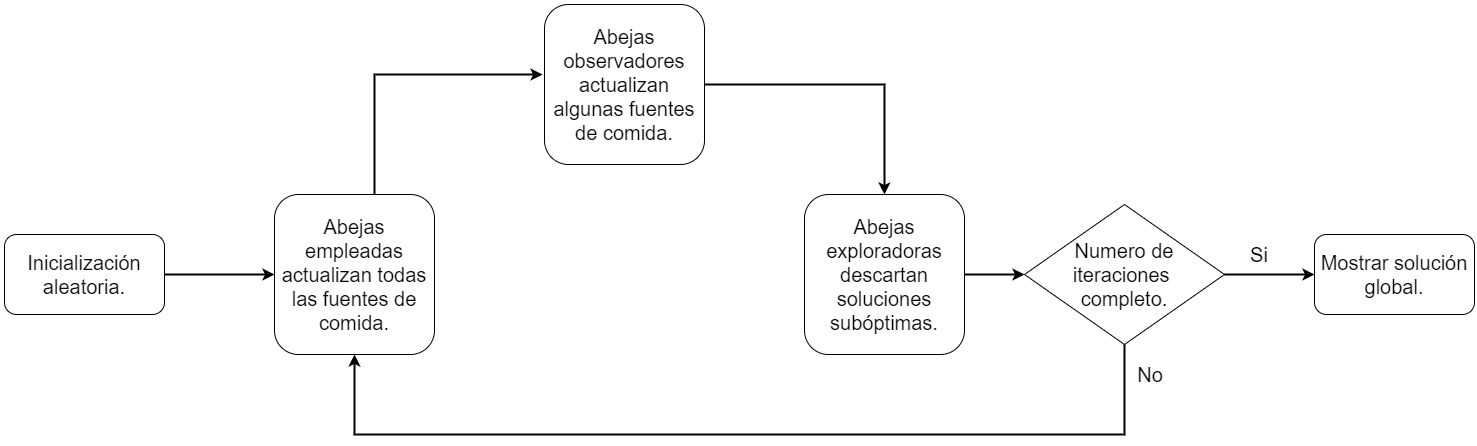
\includegraphics[scale=0.28]{flujo.png}}
        \caption{Flujo de ejecici'on.}
        \label{fig:flujo}
    \end{figure}




    \section{Resultados.}

    Se realizaron pruebas para tableros de longitud $8 \times 8$, $12\times 12$ y $16 \times 16$ (cinco ensayos por cada uno) con posicione aleatorias.
    Las medias aritm'eticas tanto del tiempo de ejecuci'on como la longitud del camino m'as largo encontrado se
    presentan en las siguientes gr'aficas.

    El algoritmo Artificial Bee Colony se ejecut'o con 32 fuentes de comida y 200 iteraciones.

    \begin{figure}[H]
        \centering
        \includegraphics[scale=0.5]{longitudes.jpg}
        \caption{Longitud de los caminos resultantes.}
        \label{fig:longitudes}
    \end{figure}

    \begin{figure}[H]
        \centering
        \includegraphics[scale=0.5]{tiempos.jpg}
        \caption{Tiempos de ejecici'on de las pruebas.}
        \label{fig:tiempos}
    \end{figure}



    \section{Conclusiones.}
    Como podemos observar en los resultados,
    de los  dos m'etodos que se presentaron como alternativa
    fue la implementaci'on de la heur'istica de Warnsdorff la que dio mejores resultados,
    encontrando caminos m'as largos que ABC y en menos tiempo. \\

    La diferencia en la calidad de las soluci'on fue bastante significativa. Aunque los tiempos de ABC dependan directamente de las iteraciones
    y fuentes de comida, los tiempos con par'ametros moderados crecen de manera mucho m'as r'apida a comparaci'on de la
    heur'istica.


    \section{Trabajo futuro.}
    Aunque los resultados obtenidos con el algoritmo ABC no son satisfactorios muestra la explotaci'on de ciertos puntos importantes, y
    con algunas variantes se puede intentar obtener mejores soluciones. \\
    Para mejorar los resultados se deben realizar modificaciones siguiendo algunos de los siguientes puntos
    \begin{itemize}
        \item Modificar el n'umero de agentes y el n'umero de iteraciones. De manera m'as general
            encontrar las cotas apropiadas para estos
            valores dependiendo del valor de la variable N.
        \item Modificar la manera en que se comparte la informaci'on entre los agentes.
        \item Modificar el proceso de las abejas exploradoras, para tratar de extender de manera m'as inteligente
            los caminos y evitar repeticiones en la informaci'on.
    \end{itemize}

    Ambos puntos requieren un an'alisis profundo, deben ser implementados y probados
    para saber si mejoran las soluciones.
    Realizar variantes queda fuera del alcance de este proyecto pero
    deben ser tomadas en cuenta para trabajos futuros.


    \section{Detalles de la implementaci'on.}
    
    \subsection{Versi'on.}
    Todas las implementaciones presentadas fueron realizadas con SWI-Prolog 8.2.4.

    \subsection{Disponibilidad de  la implementaci'on.}

    Los archivos relacionados al proyecto se encuentran disponibles
    en el repositorio\\
    \href{https://github.com/ciencias-unam/proyecto-final-VladimirSierra }{https://github.com/ciencias-unam/proyecto-final-VladimirSierra}

    Le invitamos a leer el archivo README.md para
    conocer las instrucciones precisas de ejecuci'on.

    La estructura del proyecto es:
    \dirtree{%
    .1 proyecto-final-VladimirSierra.
    .2 reporte.
    .3 bibliography.
    .3 images.
    .3 Reporte.tex.
    .3 Reporte.pdf.
    .2 src.
    .3 BeeColony.
    .4 bee\_colony.pl.
    .3 Busqueda.
    .4 heuristic\_solution.pl.
    .4 simple\_solution.pl.
    .2 README.md.
    }

    En la carpeta \textit{ reporte } se encuentra el c'odigo fuente del reporte y su correspondiente pdf. \\
    En la carpeta \textit{src/BeeColony} se encuentran los archivos de la implementaci'on para ABC. \\
    En la carpeta \textit{ src/Busqueda } se encuentran dos archivos, uno que implementa la b'usqueda completa (\textit{simple\_solution.pl}), y otro que implementa
    la b'usqueda con heur'istica (\textit{heuristic\_solution.pl}).



    %- Bibliografia
    \printbibliography

\end{document}